\documentclass[oneside, 11pt]{article}

\usepackage[T1]{fontenc}
\usepackage[utf8]{inputenc}
\usepackage[dutch]{babel}

\usepackage{fouriernc}
\usepackage[detect-all, load-configurations=binary,
            separate-uncertainty=true, per-mode=symbol,
            retain-explicit-plus, range-phrase={ tot }]{siunitx}

\usepackage{setspace}
\setstretch{1.2}

\setlength{\parskip}{\smallskipamount}
\setlength{\parindent}{0pt}

\usepackage{geometry}
\geometry{marginparwidth=0.5cm, verbose, a4paper, tmargin=3cm, bmargin=3cm, lmargin=2cm, rmargin=2cm}

\usepackage{float}

\usepackage[fleqn]{amsmath}
\numberwithin{equation}{section}
\numberwithin{figure}{section}

\usepackage{graphicx}
\graphicspath{{Figures/}}
\usepackage{subfig}

\usepackage{tikz}
\usetikzlibrary{plotmarks}

\usepackage{fancyhdr}
\pagestyle{fancy}
\fancyhf{}
\rhead{\thepage}
\renewcommand{\footrulewidth}{0pt}
\renewcommand{\headrulewidth}{0pt}

\usepackage{relsize}
\usepackage{xspace}
\usepackage{url}

\newcommand{\figref}[1]{Figuur~\ref{#1}}

\newcommand{\hisparc}{\textsmaller{HiSPARC}\xspace}
\newcommand{\kascade}{\textsmaller{KASCADE}\xspace}
\newcommand{\sapphire}{\textsmaller{SAPPHiRE}\xspace}
\newcommand{\jsparc}{\textsmaller{jSparc}\xspace}
\newcommand{\hdf}{\textsmaller{HDF5}\xspace}
\newcommand{\aires}{\textsmaller{AIRES}\xspace}
\newcommand{\csv}{\textsmaller{CSV}\xspace}
\newcommand{\python}{\textsmaller{PYTHON}\xspace}
\newcommand{\corsika}{\textsmaller{CORSIKA}\xspace}
\newcommand{\labview}{\textsmaller{LabVIEW}\xspace}
\newcommand{\daq}{\textsmaller{DAQ}\xspace}
\newcommand{\adc}{\textsmaller{ADC}\xspace}
\newcommand{\adcs}{\textsmaller{ADC}s\xspace}
\newcommand{\Adcs}{A\textsmaller{DC}s\xspace}
\newcommand{\hi}{\textsc{h i}\xspace}
\newcommand{\hii}{\textsc{h ii}\xspace}
\newcommand{\mip}{\textsmaller{MIP}\xspace}
\newcommand{\hisparcii}{\textsmaller{HiSPARC II}\xspace}
\newcommand{\hisparciii}{\textsmaller{HiSPARC III}\xspace}
\newcommand{\pmt}{\textsmaller{PMT}\xspace}
\newcommand{\pmts}{\textsmaller{PMT}s\xspace}

\DeclareSIUnit{\electronvolt}{\ensuremath{\mathrm{e\!\!\:V}}}

\DeclareSIUnit{\unitsigma}{\ensuremath{\sigma}}
\DeclareSIUnit{\mip}{\textsmaller{MIP}}
\DeclareSIUnit{\adc}{\textsmaller{ADC}}

\DeclareSIUnit{\gauss}{G}
\DeclareSIUnit{\parsec}{pc}
\DeclareSIUnit{\year}{yr}



\title{Notebooks voor Python}
\author{N.G. Schultheiss}
\docwerkblad{9}{NB}
\version{1.0}

\begin{document}

\maketitle

\section{Inleiding}

Een aantal programma's voor standaard \hisparc gegevensverwerking is voor de gebruiker onzichtbaar
en draait op de achtergrond. Specifieke software voor interpretatie van meetgegevens kan direct in
Python\footnote{Documentatie is te vinden op \url{http://docs.hisparc.nl/}} geschreven worden.

De benodigde kennis voor het schrijven van \python software is in een aantal interactieve werkbladen
 (notebooks) beschreven. Deze notebooks geven voorbeelden voor:
\begin{itemize}
\item Het ophalen van meetgegegevens.
\item Het ophalen van stationsgegevens.
\item Het verwerken van de opgehaalde gegevens
\end{itemize}
De notebooks maken gebruik van het iets uitgebreidere iPython.

\section{Software-installatie}

Voordat notebooks kunnen worden gebruikt, installeren we \python 2.7. Onder windows hebben we de keuze uit:
\begin{itemize}
\item Python(xy) (\url{https://python-xy.github.io/downloads.html})
\item WinPython (\url{https://github.com/winpython/winpython/wiki/Installation})
\end{itemize}

WinPython werkt alleen maar onder Windows. WinPython bevat onder andere de module notebook.

Onder andere operating systemen, maar eventueel ook onder Windows, is het flexibeler Python(xy) te installeren.
Om in Python(xy) notebooks te kunnen gebruiken moet {\tt pip install notebook} in een command-scherm worden
gedraaid.

De procedure voor de installatie van WinPython is alsvolgt:
\begin{itemize}
\item Download WinPython 2.7.10 en plaats de .exe op de desktop of in een mapje (Notebooks?).
\item Voer het exe-bestand uit. Er verschijnt een map WinPython.
\item Open de map WinPython. Hierin zit `WinPython Command Prompt'. Open deze en type:
 {\tt pip install hisparc-sapphire}. Druk op `Enter'. De benodigde \hisparc software wordt ge\"{i}nstalleerd.
 Ook in een Python(xy) omgeving moet sapphire worden ge\"{i}nstalleerd.
\item In de map WinPython zit verder een map `notebooks' waarin een map 'docs' zit. In deze map kunnen notebooks,
te herkennen aan het achtervoegsel {\tt ipynb}, worden geplaatst.
Op \url{https://github.com/HiSPARC/infopakket/tree/master/notebooks} zijn de hisparc notebooks op te halen. Klik
op de `RAW' knop en kopieer het bestand (rechtsklikken etc.) naar de map `WinPython\textbackslash
notebooks\textbackslash docs'.
\item Het een en ander is te testen door `Jupyter Notebook', te vinden in de `WinPython map', te draaien. De browser
opent met een scherm waarop 'docs' te zien is. Klik je op `docs' dan worden onder andere de opgehaalde notebooks
getoond. Deze zijn weer te openen door er op de klikken. Je krijgt voor ieder geopend notebook een nieuw tabblad.
\item De notebooks zijn interactief en `Shift + Enter' voert de opdrachten in de code-cellen uit. Deze zijn te herkennen aan
een opdracht prompt met een cijfer.
\end{itemize}

\section{Het gebruik van notebooks}

\begin{figure}[H]
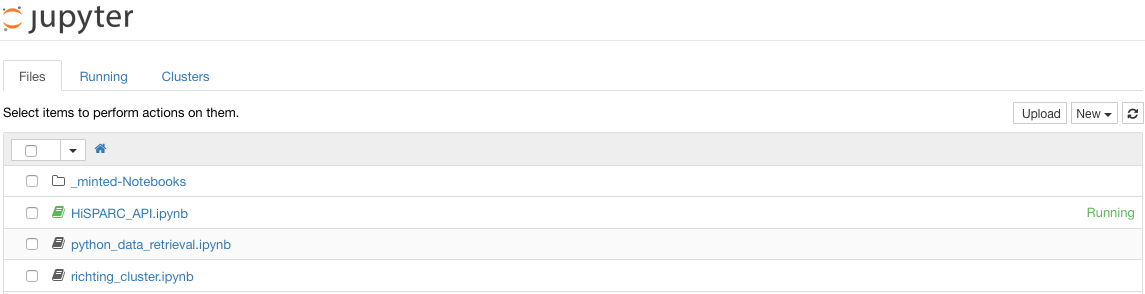
\includegraphics[width=16cm]{home.png}
\caption{Het `Home' tabblad. Er draait een virtuele computer voor het tabblad `HiSPARC-API'. Dit is onder andere te zien
aan het groene notebook icoontje.}
\end{figure}

Op de achtergrond draait een virtuele computer waarin de informatie voor
een notebook wordt beheerd. Als er twee notebooks draaien, zijn er dus ook twee virtuele computers bezig. Op het
`Home' tabblad is te zien welke computer wat doet. De virtuele computers zijn ook uit te zetten. Vink het hokje aan of
klik op het groene notebook icoontje en boven verschijnt een oranje knop `shutdown'. Hiernaast staat dan overigens
een rode vuilnisbak.

Een notebook wordt geopend door in het `Home' tabblad op de naam van het notebook te klikken. Het geopende notebook
is een interactieve leeromgeving, Er zijn cellen met uitleg en code-cellen, deze werken als terminal.

Een code-cel kan worden geselecteerd door in de code-cel te klikken. Met de toetsencombinatie `Shift + Enter' wordt de code uitgevoerd. Zo nodig
is de code aan te passen. De nieuwe code wordt weer met `Shift + Enter' uitgevoerd.

Let op: Alleen opdrachten die al met `Shift + Enter' geactiveerd zijn, zijn door de virtuele computer uitgevoerd. Foutmeldingen
worden direct gegenereerd. Zijn in dit geval alle voorgaande cellen al geactiveerd?

\begin{figure}[H]
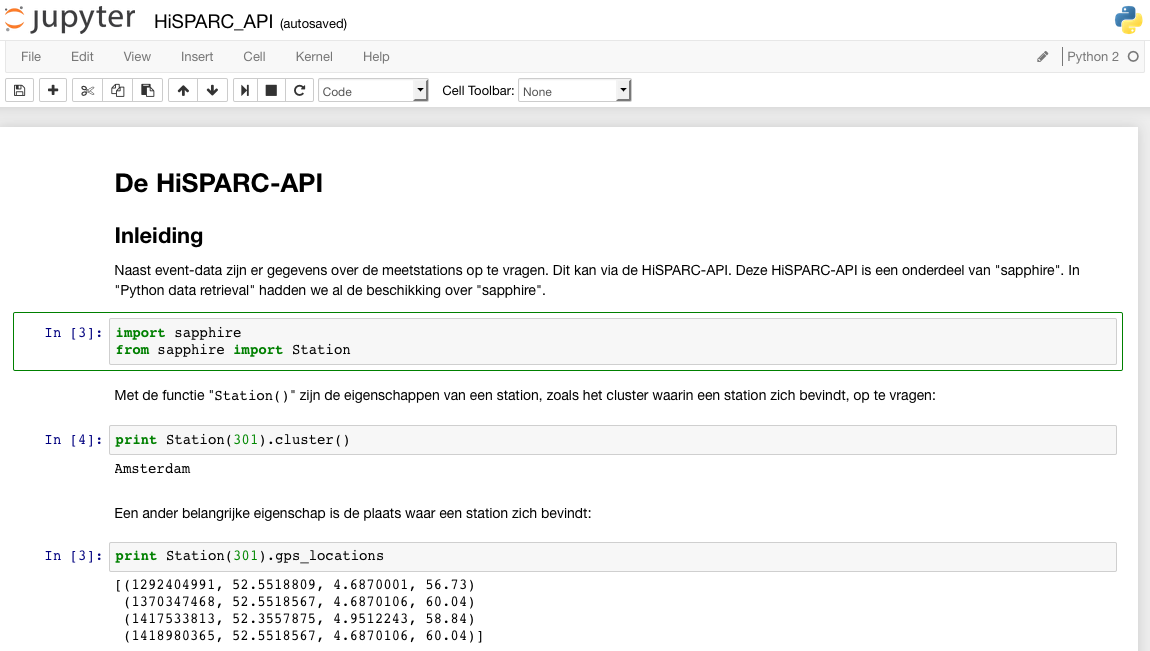
\includegraphics[width=16cm]{HiSPARC_API.png}
\caption{Het `HiSPARC-API' tabblad. Zoals aan de nummers van de opdracht prompts te zien is, zijn de eerste twee opdrachten
een extra keer gedraaid. De derde opdracht is nog niet uitgevoerd. De afgedrukte locaties zijn dus met oude data gemaakt.}
\end{figure}

De door \hisparc gepubliceerde notebooks geven een aardige start voor het verwerken van gegevens met \python.
Eventueel is na deze start een eigen notebook te maken, dit kan door op de `New' knop rechts boven in het tabblad 'Home' te
klikken. Het nieuwe tabblad heeft dezelfde kop, middenin is een pulldown menu te zien. De notebooks gebruiken de opties:

\begin{itemize}
\item Code: Hier wordt een code-cel mee gemaakt.
\item Markdown: Hier is verklarende tekst te typen. Deze voldoet aan het Markdown protocol. Dubbelklikken op een Markdown-cel
toont de broncode van de cel. `Shift + Enter' laat de cel met layout weer zien.
\end{itemize}

Bij het schrijven van een eigen notebook kunnen de volgende trefwoorden als bij het googelen nuttig zijn:

\python, NumPy, SciPy, matplotlib, list, array, Markdown, \hisparc, \sapphire, GitHub.

Internet is groot en beantwoordt veel vragen. Kritisch denken blijft van belang.

Na afloop wordt `Jupyter Notebook' afgesloten door
het terminal-venster van het begin te selecteren en op `Control + C' te drukken.

\end{document}
